%%%%%%%%%%%%%%%%%%%%%%%%%%%%%%%%%%%%%%%%%
% Friedrich M. Grabner
% CFD Coursework 2
%
%%%%%%%%%%%%%%%%%%%%%%%%%%%%%%%%%%%%%%%%%

%----------------------------------------------------------------------------------------
%	PACKAGES AND DOCUMENT CONFIGURATIONS
%----------------------------------------------------------------------------------------
\documentclass[10pt, a4paper]{article}
\usepackage{amsmath, amsthm, amssymb}
\usepackage{graphicx} % Required for the inclusion of images
\usepackage{natbib} % Required to change bibliography style to APA
\usepackage{nomencl}
\usepackage{setspace}
\usepackage{geometry} 
\usepackage{hyperref}
\usepackage{subcaption}

\geometry{a4paper,total={170mm,257mm},left=20mm,top=20mm}



\setlength\parindent{5pt} % Removes all indentation from paragraphs
\graphicspath{{./images/}}
\DeclareGraphicsExtensions{.pdf,.PDF,.jpg,.JPG,.bmp,.png,.eps,.EPS}

%\usepackage{times} % Uncomment to use the Times New Roman font

\input{/home/friedrich/ownCloud/latex/symbols.tex}
%----------------------------------------------------------------------------------------
%	DOCUMENT INFORMATION
%----------------------------------------------------------------------------------------
\newcommand*{\plogo}{\fbox{$\mathcal{PL}$}}

\newcommand*{\titleGM}{\begingroup % Create the command for including the title page in the document
\hbox{ % Horizontal box
\hspace*{0.2\textwidth} % Whitespace to the left of the title page
\rule{1pt}{\textheight} % Vertical line
\hspace*{0.05\textwidth} % Whitespace between the vertical line and title page text
\parbox[b]{0.75\textwidth}{ % Paragraph box which restricts text to less than the width of the page

{\noindent\Huge\bfseries CFD Assignment 2 \\[0.5\baselineskip] AEM-ADV19}\\[2\baselineskip] % Title
{\Large \textsc{Friedrich M. Grabner - 01220997}}\\[4\baselineskip] % Tagline or further description
{\large } % Author name

\vspace{0.5\textheight} % Whitespace between the title block and the publisher
{\noindent Imperial College London - Department of Aeronautics}\\[\baselineskip] % Publisher and logo
}}
\endgroup}
%----------------------------------------------------------------------------------------
%	TITLE PAGE
%----------------------------------------------------------------------------------------
\begin{document}
\titleGM
%----------------------------------------------------------------------------------------
%	QUESTION 1
%----------------------------------------------------------------------------------------
\section*{Question 1}
%\textbf{Run a first simulation with $Re = 200$ (line 646 of the \url{2D_compressible.f90} file) and $n_x \times n_y = 129 \times 129$ for $n_t = 10000$ time steps with a second order Adams-Bashforth scheme (itemp=1) and a CFL equal to 0.25. Generate 4 visualisations of the vorticity field for $n_t = 2500, 5000, 7500, 10000$. Briefly comment on the results in less than 100 words. (Note : The code should be configured for this question, no changes are needed).}

\noindent
\newline
In figure \ref{fig:q1} snapshots of the heat exchanger at intervals of $625$ units of normalised time are shown. Image $(a)$, the flow enters the left side of the domain at $x = 0$, a stagnation point is seen to form on the cylinder leading edge. As time passes and the flow begins to have large-scale coherent structures such as in a Von K\'{a}rm\'{a}n street vortex\cite{Karman_1963}. This can be identified in images $(a)$ and $(b)$, with small pockets of reverse flow present at each trailing edge.

The vortices now traverse the domain and inevitably collide with the cylinders that are situated downstream, image $(c)$. Then in the following image $(d)$ they are seen to wrap around the heat exchangers.

The highly vortical structures will have consequences for the convection and conduction of heat between the elements and the fluid within in the exchanger. Strong vortices will enhance the transport of fluid to the elements increase the conduction. Then the destruction of strong coherent formations will enhance the mixing of the heat throughout the fluid.

\begin{figure}[htb!]
\centering
\begin{subfigure}{.5\textwidth}
  \centering
  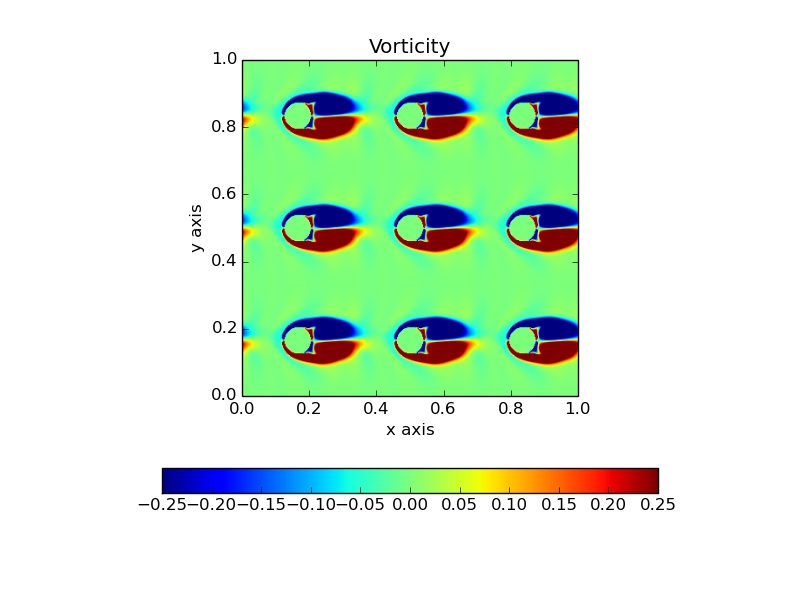
\includegraphics[width=1.1\linewidth, clip=true, trim=1cm 2cm 1cm 1cm]{q1_0001}
  \caption{$n_t = 2500$}
\end{subfigure}%
\begin{subfigure}{.5\textwidth}
  \centering
  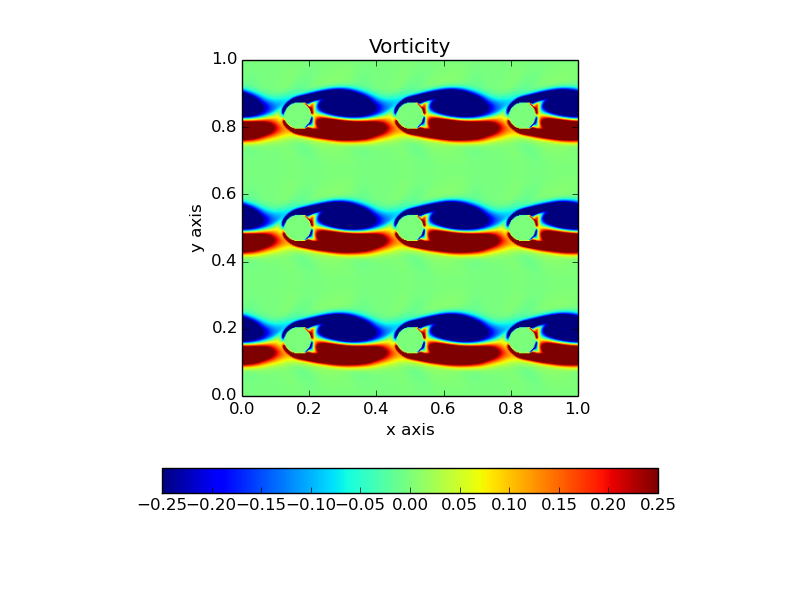
\includegraphics[width=1.1\linewidth, clip=true, trim=1cm 2cm 1cm 1cm]{q1_0002}
  \caption{$n_t = 5000$}
\end{subfigure}
\newline
\begin{subfigure}{.5\textwidth}
  \centering
  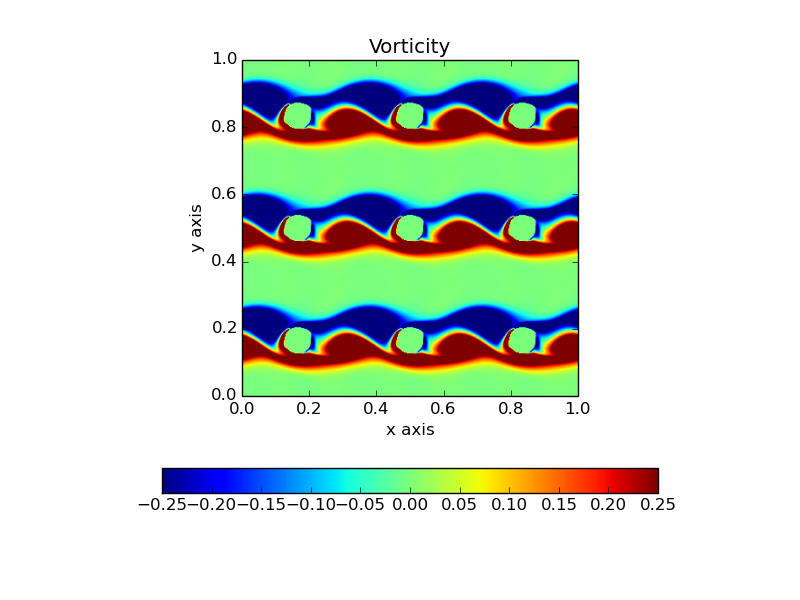
\includegraphics[width=1.1\linewidth, clip=true, trim=1cm 2cm 1cm 1cm]{q1_0003}
  \caption{$n_t = 7500$}
\end{subfigure}%
\begin{subfigure}{.5\textwidth}
  \centering
  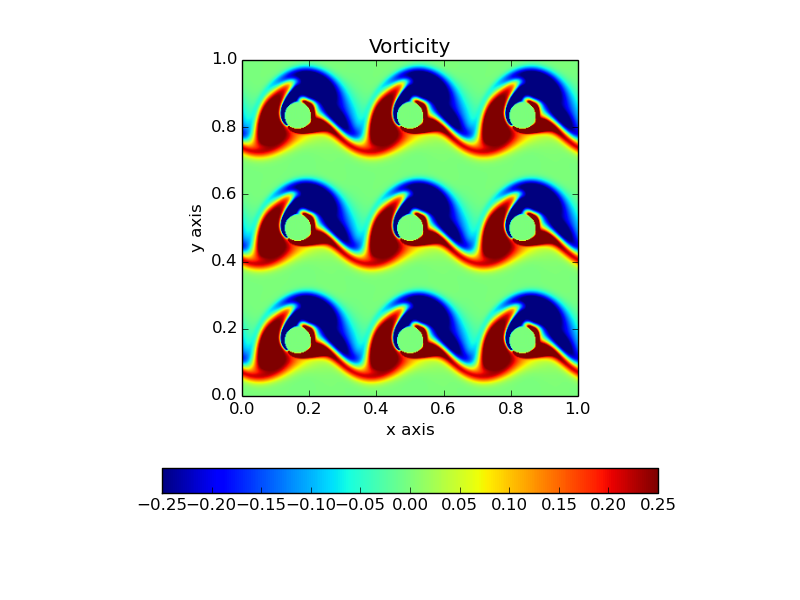
\includegraphics[width=1.1\linewidth, clip=true, trim=1cm 2cm 1cm 1cm]{q1_0004}
  \caption{$n_t = 10000$}
\end{subfigure}
\caption{Vorticity plots, CFL = 0.25, Adams-Bashford Scheme, 2\textsuperscript{nd} order accuracy derivatives.}
\label{fig:q1}
\end{figure}

%----------------------------------------------------------------------------------------
%	QUESTION 2
%----------------------------------------------------------------------------------------
\newpage
\section*{Question 2}
%\textbf{We want to increase the CFL number in order to reduce the cost of the simulation. Using the same second order Adams-Bashforth scheme (\url{itemp=1}), is it possible to run a simulation with a CFL of $0.75$? If yes, generate 4 visualisations of the vorticity field for $n_t = 2500, 5000, 7500, 10000$ and briefly comment on the results in less than 100 words. If not, try to explain why in less than 100 words.}

\noindent
\newline
It is not possible to run the simulations with $CFL = 0.75$ using the Adams-Bashforth scheme. This is due to the numerical domain no longer containing the physical domain. The solution then accumulates errors which lead to the exponential growth of values throughout the domain. Hence NaN is found at all points within the domain after 44 iterations.
%----------------------------------------------------------------------------------------
%	QUESTION 3
%----------------------------------------------------------------------------------------
\newpage
\section*{Question 3}
%\textbf{Complete the subroutine \url{rkutta} in which a third-order Runge-Kutta scheme will be used for the me advancement (use the skeleton provided in the code). The scheme is described in sec on 4.3. Run a simulation with the same parameters as in the first simulation but with a $CFL=0.75$ and the newly implemented third-order Runge-Kutta scheme ($itemp=2$, line 38 of the \url{2D_compressible.f90} file)). Generate 4 visualisations of the vorticity field for $nt = 2500, 5000, 7500, 10000$. Briefly comment on the results in less than 100 words and copy-paste the subroutine \url{rkutta} in your report.}

\noindent
\newline
Using the Runge-Kutta scheme the simulation is now stable for $CFL=0.75$. Hence for each time-step completed using this order of $CFL$, we would have required three iterations if the $CFL$ were at $0.25$. This is noted in comparison of the figure \ref{fig:q1} $(c)$ to that of figure \ref{fig:q3} $(a)$ which occur after the same period of time is simulated.

In figure \ref{fig:comp_rkadm} we can see the centre-line velocity at $nt = 2500$ and $7500$ for the Runge-Kutta simulation with $CFL =  0.75$, and the Adams-Bashforth at $CFL = 0.25$ repsectively. Both have the identical velocity therefore we can see that the more stable scheme allows us to progress in time more rapidly. Thus we understand one of the key compromises in CFD, computation time against computational accuracy.

\begin{figure}[!htb]
\centering
\begin{subfigure}{.5\textwidth}
  \centering
  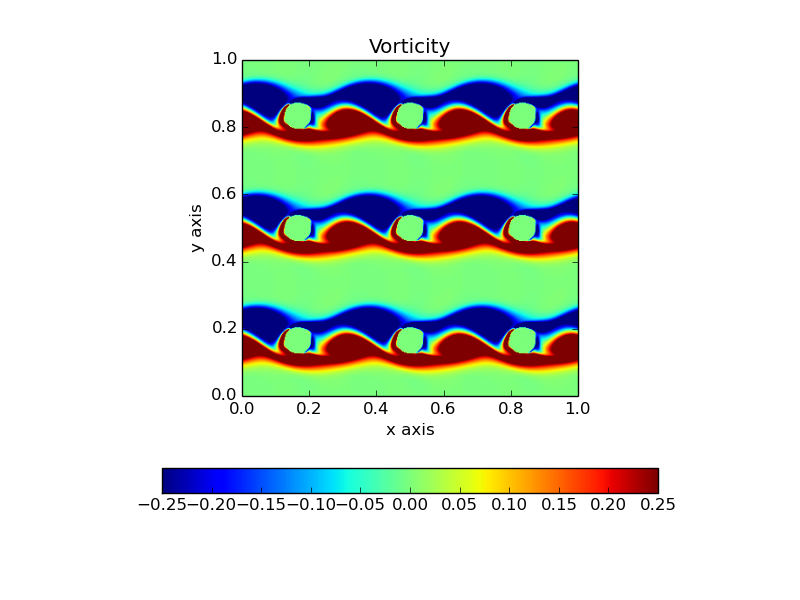
\includegraphics[width=1.1\linewidth, clip=true, trim=1cm 2cm 1cm 1cm]{q3_0001}
  \caption{$n_t = 2500$}
\end{subfigure}%
\begin{subfigure}{.5\textwidth}
  \centering
  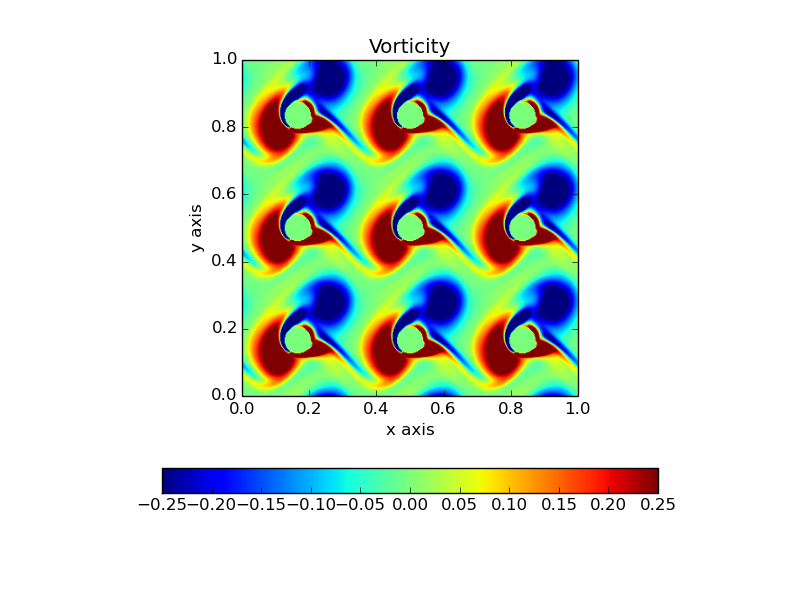
\includegraphics[width=1.1\linewidth, clip=true, trim=1cm 2cm 1cm 1cm]{q3_0002}
  \caption{$n_t = 5000$}
\end{subfigure}
\newline
\begin{subfigure}{.5\textwidth}
  \centering
  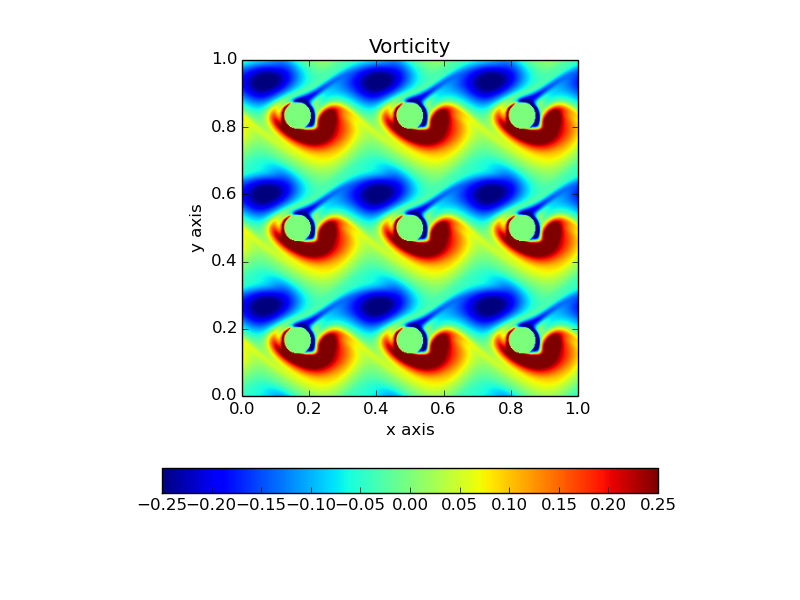
\includegraphics[width=1.1\linewidth, clip=true, trim=1cm 2cm 1cm 1cm]{q3_0003}
  \caption{$n_t = 7500$}
\end{subfigure}%
\begin{subfigure}{.5\textwidth}
  \centering
  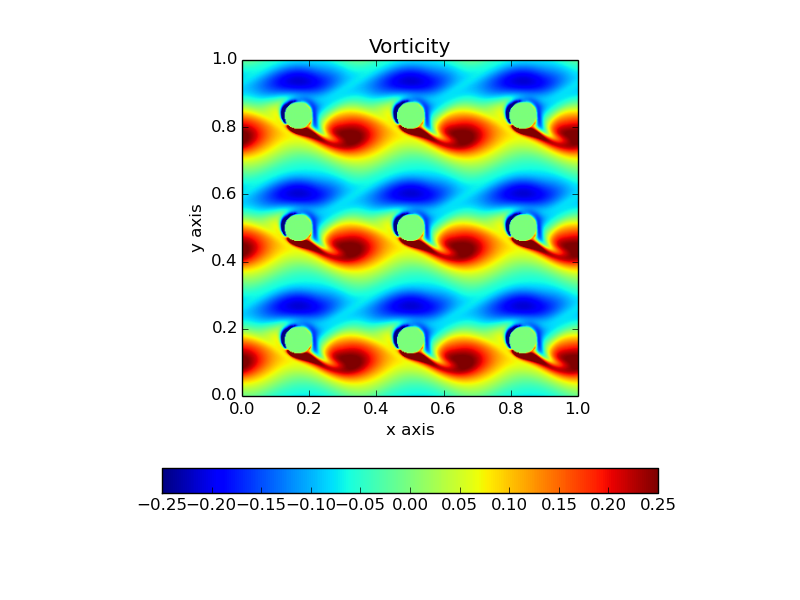
\includegraphics[width=1.1\linewidth, clip=true, trim=1cm 2cm 1cm 1cm]{q3_0004}
  \caption{$n_t = 10000$}
\end{subfigure}
\caption{Vorticity plots, CFL = 0.75, 3\textsuperscript{rd} order Runge-Kutta Scheme, 2\textsuperscript{nd} order accuracy derivatives.}
\label{fig:q3}
\end{figure}

Remarking on the development of the flow the strength of vortices decays significantly between images $(a)$ and $(d)$. This is caused by the destruction of the large coherent vortices by the heating elements. The vortices then spread and mix throughout the domain. The negative clock-wise vortex is travelling upwards in the y axis and will ultimately come into contact with the counter-clockwise vortex where they will interact further losing kinetic energy.

\begin{figure}[!htb]
  \centering
	  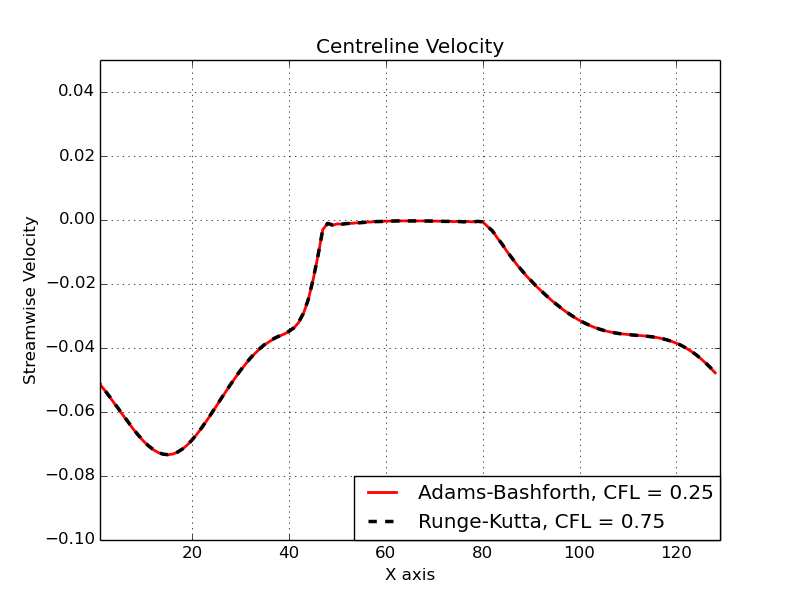
\includegraphics[width=.45\linewidth, clip=true, trim=0cm 0cm 0cm 0cm]{velocity}
  \caption{Comparison of centreline velocity at identical simulation time intervals $t = 1875 units$.}
  \label{fig:comp_rkadm}
\end{figure}%

%----------------------------------------------------------------------------------------
%	QUESTION 4
%----------------------------------------------------------------------------------------
\newpage
\section*{Question 4}
%\textbf{Instead of circular cylinders, run a simulation using the same parameters as in the first simulation (second order Adams-Bashforth scheme, \url{itemp=1}, $CFL=0.25$) but with square cylinders. The subroutine \url{initl} needs to be modified, in particular for the array \url{eps}. For example, you can define \url{imin},\url{imax},\url{jmin},\url{jmax} where (\url{imin},\url{jmin}) is the bottom left corner of the square, (\url{imin},\url{jmax}) the bottom right corner, (\url{imax},\url{jmin}) the top left corner and (\url{imax},\url{jmax}) the top right corner. The length of the square will be equal to the diameter d of the circular cylinder. Generate 4 visualisations of the vortcity field for $nt = 2500, 5000, 7500, 10000$. Copy-paste the new 2D loop for the square cylinder in your report and briefly comment on the results in less than 50 words.}

The square cylinders are shown in figure \ref{fig:q4}. The vorticity plots are very similar to those of the circular cylinders. However we can see the inner trailing vortex is far weaker than for circle. This is as there is no adverse pressure gradient to allow the grouth of these counter rotating structures. This has the effect of increasing the strength of the large vortices which then begin to interact with the other cylinders downstream. Overall the solution has stronger and more distinct separated vortices, but shares similar general characteristics of shear layer mixing as with the circular case.

\begin{figure}[htb!]
\centering
\begin{subfigure}{.5\textwidth}
  \centering
  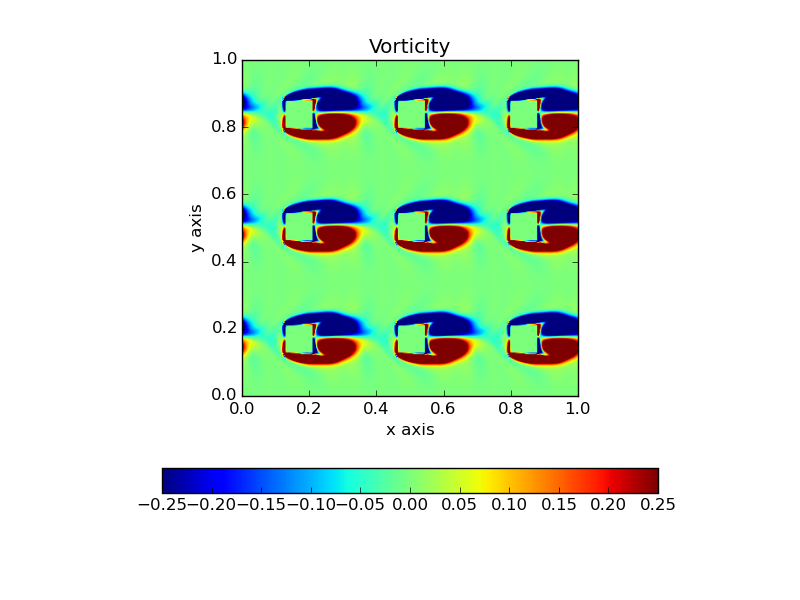
\includegraphics[width=1.1\linewidth, clip=true, trim=1cm 2cm 1cm 1cm]{q4_0001}
  \caption{$n_t = 2500$}
  \label{fig:sub1}
\end{subfigure}%
\begin{subfigure}{.5\textwidth}
  \centering
  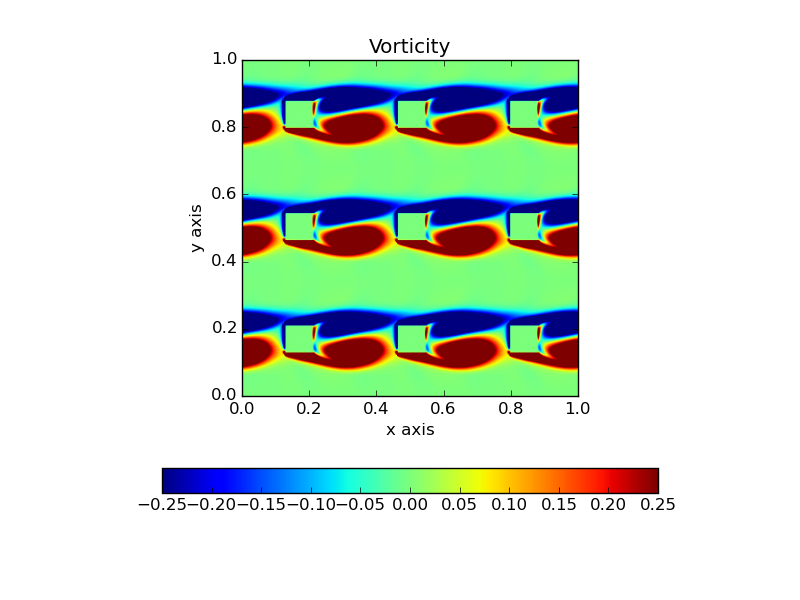
\includegraphics[width=1.1\linewidth, clip=true, trim=1cm 2cm 1cm 1cm]{q4_0002}
  \caption{$n_t = 5000$}
  \label{fig:sub2}
\end{subfigure}
\newline
\begin{subfigure}{.5\textwidth}
  \centering
  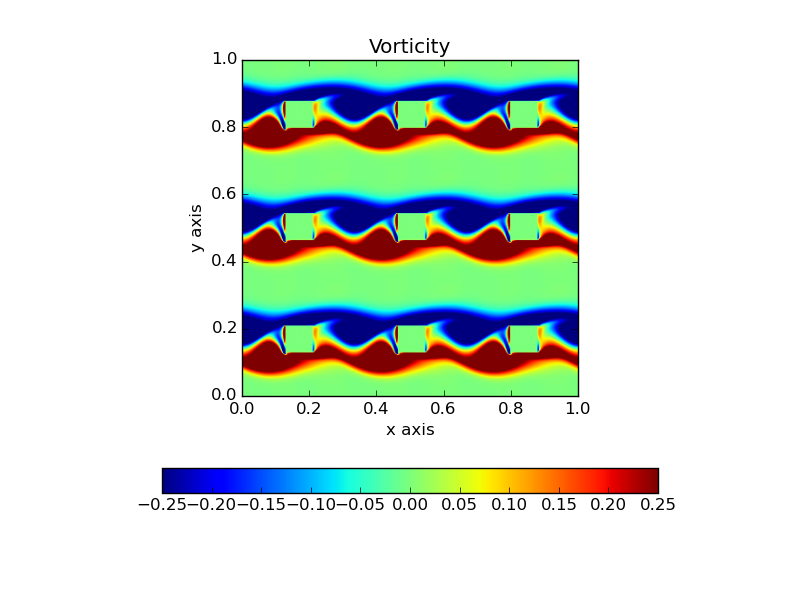
\includegraphics[width=1.1\linewidth, clip=true, trim=1cm 2cm 1cm 1cm]{q4_0003}
  \caption{$n_t = 7500$}
  \label{fig:sub1}
\end{subfigure}%
\begin{subfigure}{.5\textwidth}
  \centering
  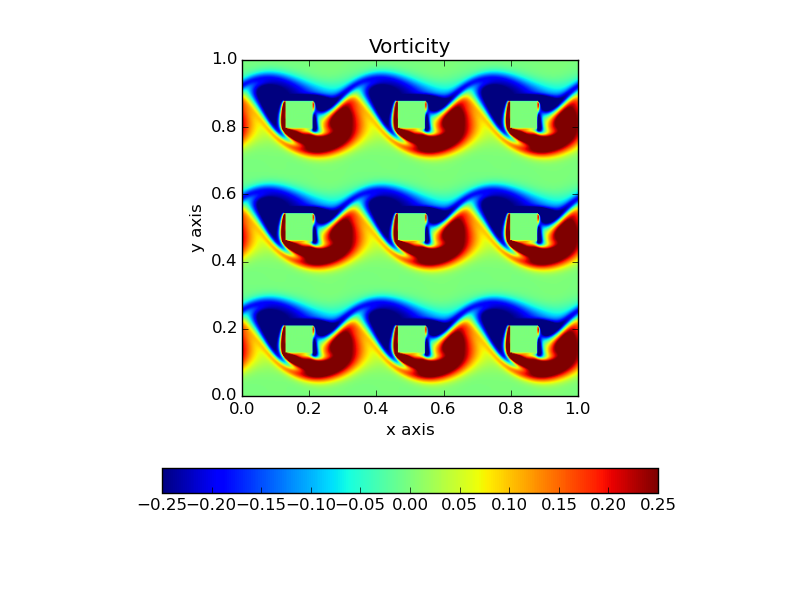
\includegraphics[width=1.1\linewidth, clip=true, trim=1cm 2cm 1cm 1cm]{q4_0004}
  \caption{$n_t = 10000$}
  \label{fig:sub2}
\end{subfigure}
\caption{Vorticity plots, CFL = 0.25, 2\textsuperscript{nd} order Adams-Bashforth Scheme, 2\textsuperscript{nd} order accuracy derivatives.}
\label{fig:q4}
\end{figure}


%----------------------------------------------------------------------------------------
%	QUESTION 5
%----------------------------------------------------------------------------------------
\section*{Question 5}
%\textbf{We want to use centered fourth-order schemes for the first and second derivatives in the two spatial directions. Write four new subroutines, using the skeletons provided in the code : \url{derix4, deriy4, derxx4} and \url{deryy4}. In the subroutine \url{fluxx}, replace the second-order first and second derivatives with the new fourth-order ones. Then run a simulation with same parameters as the first simulation (question 1) but with the new the fourth-order schemes. Generate 4 visualisations of the vorticity field for $nt = 2500, 5000, 7500, 10000$. Briefly comment on the results and discuss the differences (if any) with the first simulation (question 1) in less than 100 words. Copy-paste the four new subroutines in your report.}
\noindent
\newline

Using the fourth order spatial derivatives shows no discernible difference in scheme when looking at figure \ref{fig:q5} below. Looking at the second order Taylor expansion,

\begin{equation}
\frac{\partial u}{\partial x}
   = \frac{u_{i+1} - u_{i-1}}{2 \Delta x} + \frac{u'''_{i} \Delta x^2}{6} + O(\Delta x^3)
\end{equation}  

\begin{equation}
\frac{\partial^2 u}{\partial x^2}
   = \frac{u_{i+1} - 2u_i + u_{i-1}}{\Delta x^2} - \frac{u''''_{i} \Delta x^2}{12} + O(\Delta x^3)
\end{equation}

which we can compare with the fourth order derivatives shown below.

\begin{equation}
\frac{\partial u}{\partial x}
   = \frac{-u_{i+2} + 8u_{i+1} - 8u_{i-1} + u_{i-2}}{12 \Delta x} + O(\Delta x^4)
\end{equation}

\begin{equation}
\frac{\partial^2 u}{\partial x^2}
   = \frac{-u_{i+2} + 16u_{i+1} - 30u_i + 16u_{i-1} -u_{i-2}}{12 \Delta x^2} + O(\Delta x^4)
\end{equation}

\begin{figure}[htb!]
\centering
\begin{subfigure}{.5\textwidth}
  \centering
  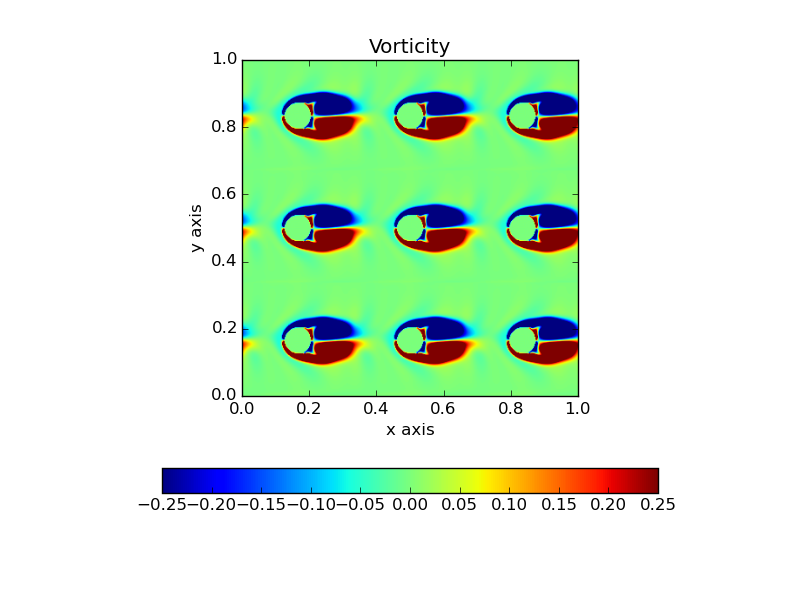
\includegraphics[width=1.1\linewidth, clip=true, trim=1cm 2cm 1cm 1cm]{q5_0001}
  \caption{$n_t = 2500$}
\end{subfigure}%
\begin{subfigure}{.5\textwidth}
  \centering
  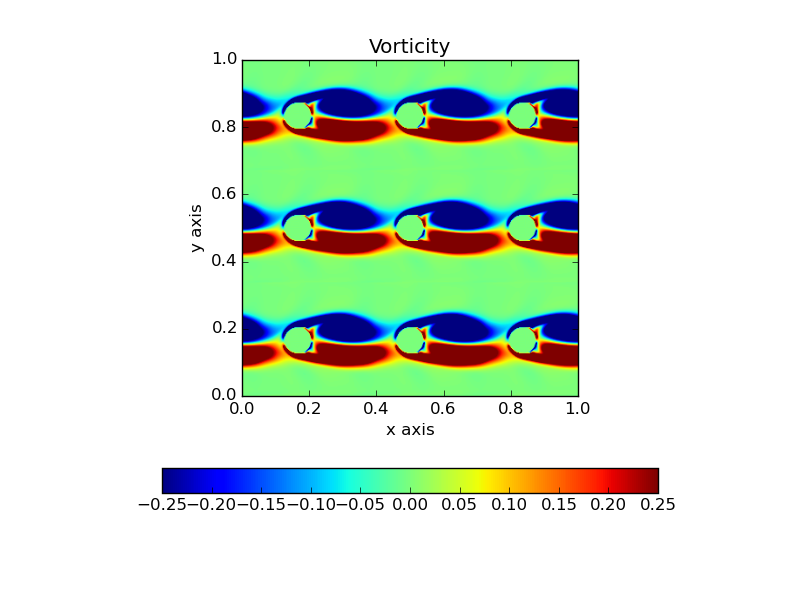
\includegraphics[width=1.1\linewidth, clip=true, trim=1cm 2cm 1cm 1cm]{q5_0002}
  \caption{$n_t = 5000$}
\end{subfigure}
\newline
\begin{subfigure}{.5\textwidth}
  \centering
  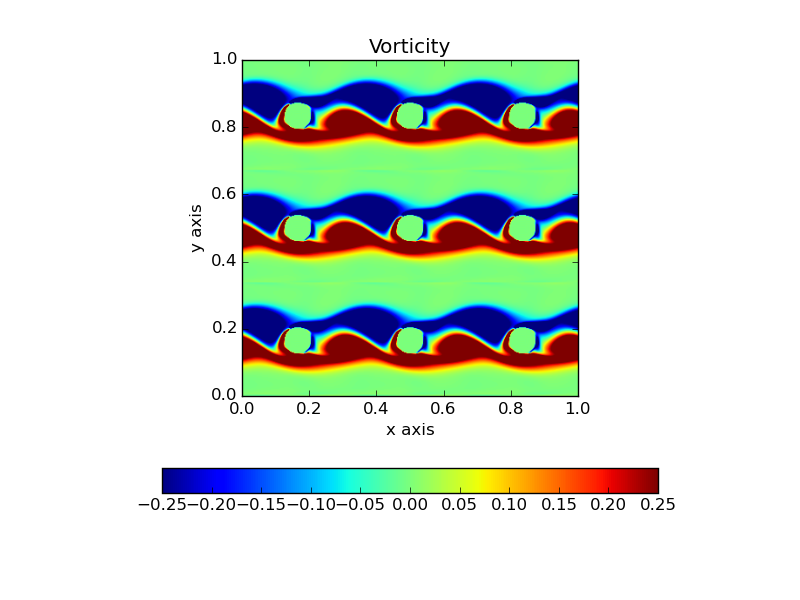
\includegraphics[width=1.1\linewidth, clip=true, trim=1cm 2cm 1cm 1cm]{q5_0003}
  \caption{$n_t = 7500$}
\end{subfigure}%
\begin{subfigure}{.5\textwidth}
  \centering
  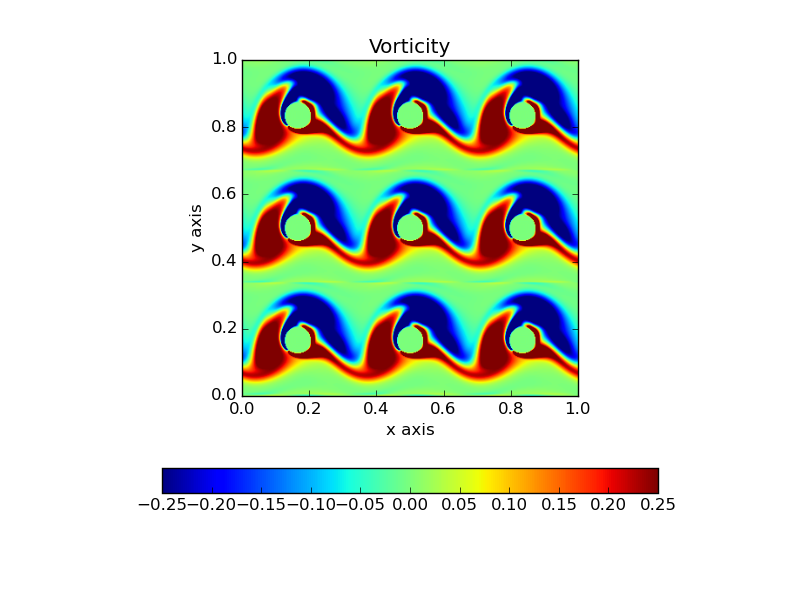
\includegraphics[width=1.1\linewidth, clip=true, trim=1cm 2cm 1cm 1cm]{q5_0004}
  \caption{$n_t = 10000$}
\end{subfigure}
\caption{Vorticity plots, CFL = 0.25, Adams-Bashford Scheme, 4\textsuperscript{th} order accuracy derivatives.}
\label{fig:q5}
\end{figure}

Plotting the centreline velocity of both the second and fourth order schemes against each other

\begin{figure}[htb!]
\centering
\begin{subfigure}{.5\textwidth}
  \centering
  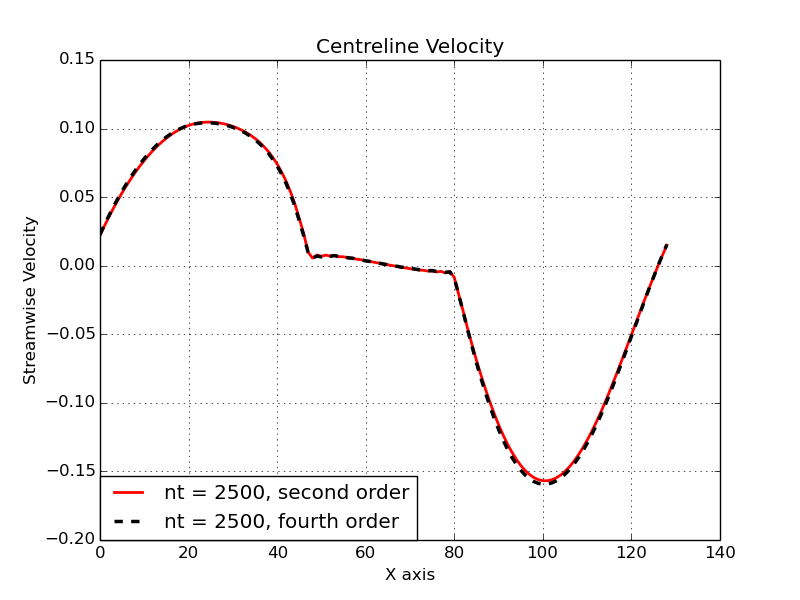
\includegraphics[width=.5\linewidth, clip=true, trim=1cm 1cm 1cm 1cm]{velocity1}
  \caption{$n_t = 2500$}
\end{subfigure}%
\begin{subfigure}{.5\textwidth}
  \centering
  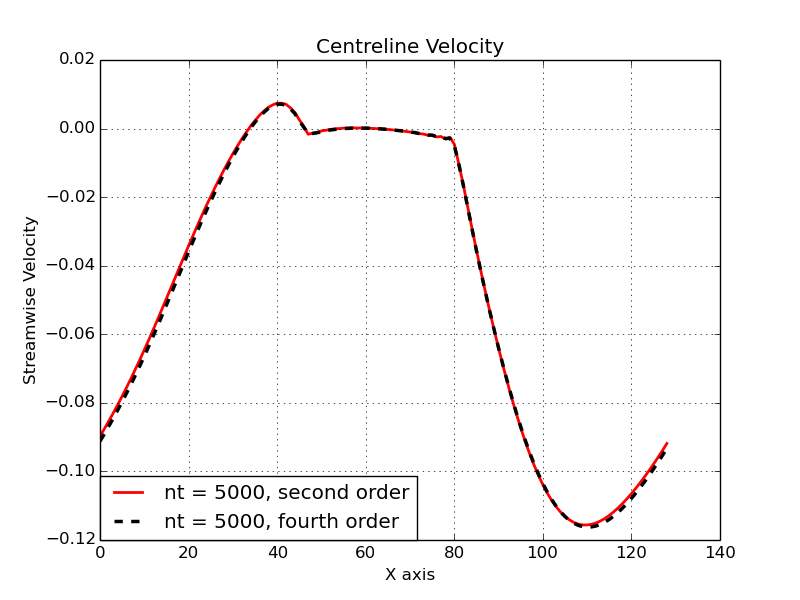
\includegraphics[width=.5\linewidth, clip=true, trim=1cm 1cm 1cm 1cm]{velocity2}
  \caption{$n_t = 5000$}
\end{subfigure}
\newline
\begin{subfigure}{.5\textwidth}
  \centering
  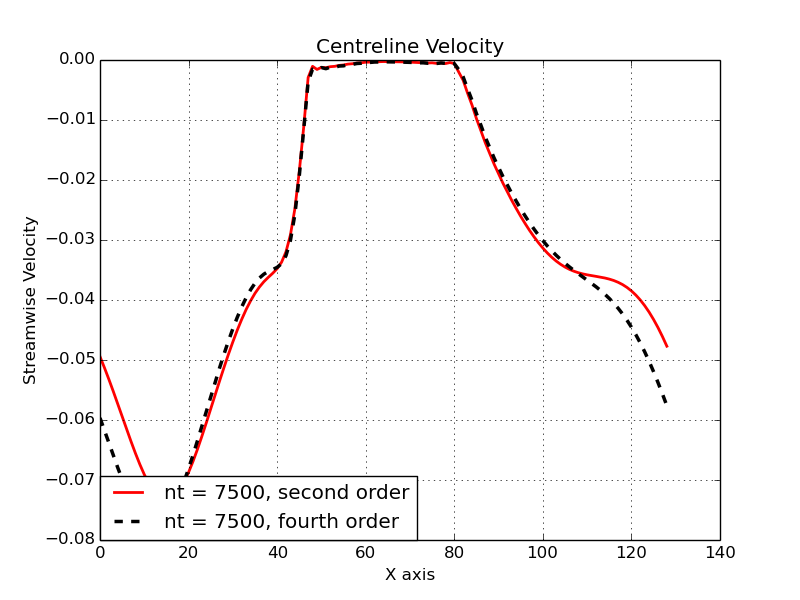
\includegraphics[width=.5\linewidth, clip=true, trim=1cm 1cm 1cm 1cm]{velocity3}
  \caption{$n_t = 7500$}
\end{subfigure}%
\begin{subfigure}{.5\textwidth}
  \centering
  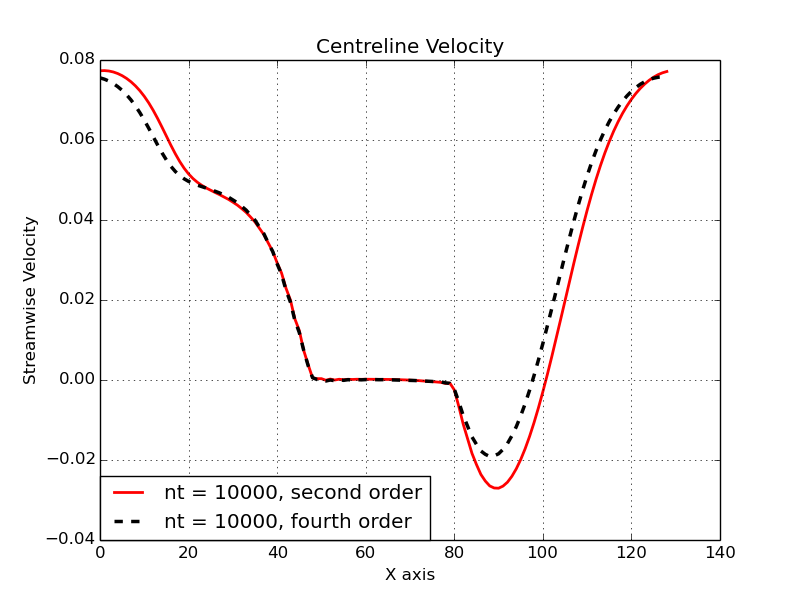
\includegraphics[width=.5\linewidth, clip=true, trim=1cm 1cm 1cm 1cm]{velocity4}
  \caption{$n_t = 10000$}
\end{subfigure}
\caption{Centerline Velocity, CFL = 0.25, Adams-Bashford Scheme.}
\label{fig:q5c}
\end{figure}

Comparison of the centerline velocity fields of the cylinders between 2\textsuperscript{nd} and 4\textsuperscript{th}, we see that there is a small difference in velocity profile however it only becomes apparent in figure \ref{fig:q5c} $(c)$ onwards. The profiles are somewhat smoothed, due to the inclusion of more points in the calculation. However from the centerline velocity alone it is not possible to say whether the 4\textsuperscript{th} or 2\textsuperscript{nd} order are more dissipative in reality. Though it is likely to be the 2\textsuperscript{nd} order version as it truncates more of the solution, and there are no discontinuities across which the larger stencil of the fourth order derivatives may lose energy mistakenly.

%----------------------------------------------------------------------------------------
%	QUESTION 6
%----------------------------------------------------------------------------------------
\section*{Question 6}
%\textbf{What will happen to the flow if you run the simulation in question 1 for a very long time? Justify your answer in less than 100 words.}

Running the simulation for a long period of time would see the decay of any flows. As the simulation adds velocity only upon initialising of the domain, the use of periodic boundary condition means there is no velocity input at inlet or outlet. Corollary to this the truncation errors behaves as a dissipative term, hence energy is removed from the domain upon each iteration. In CFD a pressure gradient is often added to periodic boundary condition problems to keep TKE (total kinetic energy) constant within the domain at each timestep.

In regards to the development of the flow, the large coherent structures would break with each interaction of the heating elements. This would cause the development of a fully turbulent flow within the domain, though the grid resolution is under-resolved to capture this. Ergo the flow would simply dissipate for this case.

%---------------------------------------------------------------------------------------
%	BIBLIOGRAPHY
% ---------------------------------------------------------------------------------------
\newpage
\bibliographystyle{unsrt}	% in order of appearance
%\bibliographystyle{acm}	% (uses file "plain.bst")
%\bibliographystyle{abbrv}	% (uses file "plain.bst")
%\bibliographystyle{siam}	% (uses file "plain.bst")
%\bibliographystyle{apalike}
\bibliography{/home/fmg215/Documents/latex/myrefs}		% expects file "myrefs.bib"}
%----------------------------------------------------------------------------------------
% END DOCUMENT
%----------------------------------------------------------------------------------------
\end{document}